\chapter{Theory}

This chapter of the report is where we lay the theroetical groundwork for the discussions and choices in the rest of the report. The choice of technologies in chapter \ref{Method}, is based on the information in this chapter. The chapter starts with some definitions and concepts and a concise summary of the ransomware threat in sections \ref{Ransomware} and \ref{Anatomy}. The technologies we utilized in the project are described in the following four sections until the last section, \ref{BestStrat} presents some so-called best practices. 

\section{Definitions and concepts}

\subsection{Public cloud}
Any search for a definition of the cloud will yield a tremendous number of results,
and just about as many different interpretations of what the cloud actually is.
In a 2010 article, Hofmann and Wood \cite{hofmann_cloud_2010} provide the following definition:
"At its core, cloud computing means providing computing services via the Internet.
The 'cloud' idea is tightly connected with the 'as a service' idea."
They go on to describe the public cloud as a set of standard resources that can be combined into applications or services. While this article is over ten years old, the fundamentals are still the same. 

The public cloud  is available to organisations and consumers through cloud platforms such as Amazon Web Services (AWS), Microsoft Azure, and Google Cloud Platform (GCP), which are the biggest providers on the market \cite{richter_amazon_2022}. Cloud platforms generally provide resources to the user. Resources are manageable items that are available through that cloud platform \cite{tfitzmac_azure_nodate}. A common example is virtual machines, that are compute resources made available to costumers as a server over the internet, but it is in fact a virtual server on top of a physical server.

\subsection{CIA-triad} \label{CIA}
An important aspect of Security design is the concept of the CIA-triad. CIA is short for: Confidentiality, Integrity, and Availability \cite{laan_it_2017}. Any security control must address either the confidentiality of the thing you  are trying to secure, or its integrity or availability. A security control is any action taken to secure something in an system. 
\begin{itemize}
    \item Confidentiality
       \newline
        This involves keeping data secret, and preventing unauthorized disclosure of data.
    \item Integrity
    \newline
    This ensures that data is not modified by unauthorized persons, or unauthorized modifications are not made to data no matter by whom. It also ensures data consistency. 
    \item Availability
    \newline
    This aspect is about making sure that data and resources are available to authorized personnel in a timely manner. 
\end{itemize}


\subsection{Ransomware}
Ransomware is a central aspect of this project and has a dedicated chapter (\ref{Ransomware}) Ransomware is a type of malware that encrypts files on an infected system and holds the files as ransom for typically large sums of money -- typically in the form of cryptocurrency. The malicious actor that spread the ransomware in question will usually have the decryption key and only share it with the victim once the ransom has been paid \cite{hassan_ransomware_2019}.

\subsection{Databases}

A database is a type of system that stores and organizes data.
Databases are used for many different purposes including storing application data, analytics, [more]
Structured Query Language (SQL) is a commonly used language for interacting with databases.
Databases that do not use SQL exist as well.
These are commonly referred to as "NoSQL" databases.

\subsection{Cryptography concepts}
One of the essential building blocks of any ransomware is the concept of cryptography. Laan defines cryptography in his book as "the practice of hiding information using encryption and decryption techniques." \cite{laan_it_2017}. Only those who know how to decrypt the information can read it. This is usually done using a cipher -- a pair of algorithms -- that along with a key -- the secret only known by the encrypter and those they share it with -- controls the encryption or decryption process. 

A number of different methods of encryption exist, some more advanced than others. For security purposes, it is generally advised to use a known cipher, with a secret key. As the cipher will be subject to scrutiny by security professionals at large, the odds of gaining any security by obfuscation in this space is limited. Given that the key can remain secret however, a tried and tested, open-source cipher method with a secret key is by far the most secure. 

\subsection{RPO and RTO} 
The efficiency of a data protection or disaster recovery plan can be 
measured by two specifications, namely;
Recovery Point Objective (RPO) and Recovery Time Objective (RTO).

\paragraph{RPO}\label{theory:rpo}
The Recovery point objective (RPO) is the data loss after disaster recovery, measured by time, upon where data loss exceeds the threshold of what an organization can accept.

\paragraph{RTO} \label{theory:rto}
Recovery Time Objective (RTO) is a metric that 
defines both the time duration within which a service must be restored to after a 
disaster in order to avoid detrimental damage caused to the business. 

\section{Ransomware}
\label{Ransomware}
\subsection{Definition}
Ransomware is a type of \gls{malware} that attempts to extort money from victims by holding their data for ransom. Access to data is typically blocked by encrypting the data (crypto ranomsware) or by locking the computer (locker ransomware) \cite{hassan_ransomware_2019}.

Recovering encrypted files is generally exceedingly difficult without access to the encryption key that was used. Paying the ransom is also not a reliable recovery option, as there is no guarantee the attacker will keep their end of the bargain. In addition, by paying the ransom the victim is likely to be marked as a target in future attacks, as well as funding the ransomware threat actor. According to reserach from Cybereason 80\% of victim organisations that paid the ransom were attacked again \cite{noauthor_new_nodate}.

\subsection{Ransomware trends}

Ransomware has been steadily on the rise and has become highly relevant for the cybersecurity industry during the late 2010s. Malware actors have become more organized, and more goal-oriented, which according to cybersecurity research group Cisco Talos means that they now primarily try to follow the money \cite{stemland_cyberkriminelle_2021}. Cisco Talos pose that threat actors do not want to risk getting discovered by installing low-profit malware, when they instead can sell the access, or use ransomware to make a larger profit. 

This explains why ransomware has grown in popularity by threat actors in recent years. According to a report by the security firm Check Point, the first half of 2021 saw twice as many known ransomware attacks compared to 2020 \cite{noauthor_new_2021}. The report also highlights some trends that further Cisco Talos’ point: Threat actors keep searching for ways to employ double- or triple-extortion techniques to maximize profits. Double- and triple-extortion involves not only extorting the victim organisation for ransom, but also threatening the organisations customers or clients and threaten to release their data unless they also pay up. 

The energy and utilities sector was also the second-most targeted, which is part of the reason for this project focusing on the needs of the Norwegian energy sector \cite{noauthor_new_2021}. Prominent examples of this are the ransomware attacks on Volue, a Norwegian company that provides technology to the energy and infrastructure sector, as well as the prolific Colonial Pipeline attack. In the latter the pipeline that supply the southeastern United States with gasoline had to stop all operation because of a ransomware attack on its computerized equipment. Both attacks occured in May 2021 \cite{stupp_energy_2021}. The latter has been named "one of the most disruptive ransomware attacks ever on US critical infrastructure" \cite{thomas_state_2021}. \label{EnergyAttacks}

The goal for any business has to be the prevention of ransomware attacks, but that may not always be possible, as with the attack on the Norwegian parliament in March 2021 \cite{noauthor_stortinget_2021}, where a \gls{zero-day} vulnerability in Microsoft Exchange proved fatal enough for data to be exfiltrated. Similar examples are prevalent, and it is impossible for an organisation to guarantee prevention. 

When prevention is not possible, the mitigation of the consequences of ransomware attacks become vital. One of the most important risk mitigation measures that an organisation can do is to set up backup solutions for their data. For critical infrastructure this backup has to both be frequent, and consistent enough to let the company return to normal operations quickly, even when they are the victim of a ransomware attack. 

\subsubsection{Human-operated ransomware}

% https://www.checkpoint.com/cyber-hub/threat-prevention/ransomware/human-operated-ransomware/
% https://www.pwc.co.uk/issues/cyber-security-services/insights/responding-to-growing-human-operated-ransomware-attacks-threat.html

% [TODO] Skriv mer

In a human-operated ransomware attack, the attacker target a specific organization,
and manually attempts to break in, gain 
A ransomware attack where  
A human-operated ransomware attack 

\subsubsection{Ransomware as a service, access as a service}

Ransomware-as-a-service (RaaS) is a business model for ransomware developers, in which the developers license their ransomware to other threat actors. According to an article published by Threatpost, ransomware gangs look more and more like legitimate businesses, with IT-support, and customer service. These ransomware gangs offer affiliate programs to whom they provide RaaS-offerings \cite{seals_2021_nodate}.

RaaS is a driving factor in today's ransomware landscape, and most ransomware gangs operate on the RaaS model, according to research from security firm Abnormal \cite{noauthor_threat_nodate}. This shows an overarching trend in the way that ransomware gangs pick their targets. Gone are the days of spreading malware to as many systems and networks as possible, hoping someone will bite. Nowadays, an attack is preceded by weeks or months of reconnaissance. Not only do the attackers explore the systems they've penetrated, but they also explore the businesses financial situation and internal communications in order to set a ransom that has the highest chance of resulting in a payout, whilst also being as large a sum as possible \cite{seals_2021_nodate}.

The model for choosing affiliates is also highly selective, and hopefuls will have to go through a rigorous application process, submitting a resume and impressing the ransomware gang in an interview. The ransomware gangs are on their hand worried about poor-performing affiliates which may compromise the brand's reputation, or western law enforcement agencies. As a result many ransomware gangs are quite picky both in terms of technical abilities, as well as language and knowledge of Russian history and culture that is not easily researched \cite{seals_2021_nodate}.

\subsection{Ransomware groups}
According to research made by Abnormal \cite{noauthor_threat_nodate}, a few ransomware gangs have dominated the ransomware scene in the last two years. These are Conti, LockBit, Pysa, REvil, and Maze/Egregor. They were responsible for more than half of all ransomware attacks in this time period. Conti, LockBit and Pysa are still active as of the publication of their research, and all have a large number of victims.

The aforementioned prolific attacks on Volue and the Colonial Pipeline (see \ref{EnergyAttacks}) were conducted by Darkside and Ryuk respectively \cite{thomas_state_2021}. Both are known for attacking the energy sector. 

\subsection{How ransomware works}
The ransomware field is ever evolving, 
and any analysis is only snapshot of ransomware at the time of publishing.
Despite this it is useful to assess the present situation to understand the threat at hand. 

An analysis of encryption schemes in modern ransomware was published in 2020 by Plozek, Svec, and Debnar \cite{ploszek_analysis_2021}. In the paper 10 different ransomware samples were analysed, but only one of those, LockBit,overlaps with the dominating groups as assessed by Abnormal. The samples were collected between 2019 and 2020, so this might show the rate of evolution in this field. 

In the analysis the researchers identified four different encryption schemes in the ransomware malware samples. The differences mainly concerned where the keys were generated, and how they are distributed. Prevalent in their findings was that different keys are usually generated for each victim, indicating that the goal no longer is to affect as many victims as possible, but to make as much profit per victim that they can \cite{ploszek_analysis_2021}.

Another major finding in their research was that malware authors are getting better at cryptography. Generally compared to older research the researchers found that modern ransomware used more secure encryption algorithms than older ransomware. This trend toward more advanced encryption schemes align with the general trend of ransomware gangs getting more professional \cite{ploszek_analysis_2021}.

This makes brute force decryption less feasible/not feasible at all, and any files encrypted by ransomware should be considered lost, as decryption of those files is not likely to have effect, especially in the time necessary for an organisation to not suffer great losses. In addition the paper discovered that several of the ransomware strains created a separate key for each encrypted file, so the brute-force method would be even less feasible \cite{ploszek_analysis_2021}.
    
\section{The anatomy of an attack} \label{Anatomy}

Cyberattacks generally follow a similar pattern,
with the same main steps or phases.
%citation needed.
The number of steps, and the names they are assigned differ,
but they are generally similar.
A brief overview of the anatomy of an attack is described below.
Figure \ref{fig:attack_anatomy} illustrates these steps visually,
as a flowchart, showing possible paths an attacker may take.

\subsubsection{Reconnaissance}
An attacker can spend a long time before an attack gathering information,
in order to evaluate which organization they should target to earn the most money,
as well as looking for vulnerabilities that can be used to gain a foothold
in the organization's network.

\subsubsection{Initial access}

After gathering information about the organization, 
the hacker will try to gain access to the network.
According to BankInfoSecurity \cite{may_29_top_nodate},
the following three attacks are the most common types of attacks used for
initial access:

\begin{itemize}
    \item RDP compromise \\
    By exploiting weak Remote Desktop Protocol (RDP) endpoints,
    a hacker can get full access to a user account on the network.
    RDP compromise is currently the most common 
    vulnerability used for initial access \cite{noauthor_remote_nodate, may_29_top_nodate}
    
    \item Phishing \\
    Phishing is a type of social engineering attack where the attacker
    sends a link or email attachment containing malware,
    pretending that it is legitimate.
    Through the information gathered in the reconnaissance step,
    the attacker may be able to craft believable emails.
    
    \item Software vulnerabilities \\
    Vulnerabilities or bugs in software can expose the organization
    in a way that an attacker can take advantage of.
\end{itemize}

\subsubsection{Expansion}

After getting a foothold in the organization's network,
the attacker will move through the network (lateral movement)
to gain information about resources and assets,
and attempt to expand their privileges (privilege escalation).

\subsubsection{Exploitation}

After gaining access to enough privileges and resources, the main attack can begin.
Before deploying the ransomware,
the attacker might first attempt to exfiltrate (steal) valuable data.
The attacker might also try to destroy backups before
proceeding to deploy the ransomware itself, encrypting the data.

After this, the attacker typically demands a ransom in order to decrypt the data.
If the data has been exfiltrated,
the attacker might try to perform a double extortion attack,
in which they make a threat to release the exfiltrated data publicly
if the organization does not pay the ransom.

\begin{figure}[h!]
    \centering
    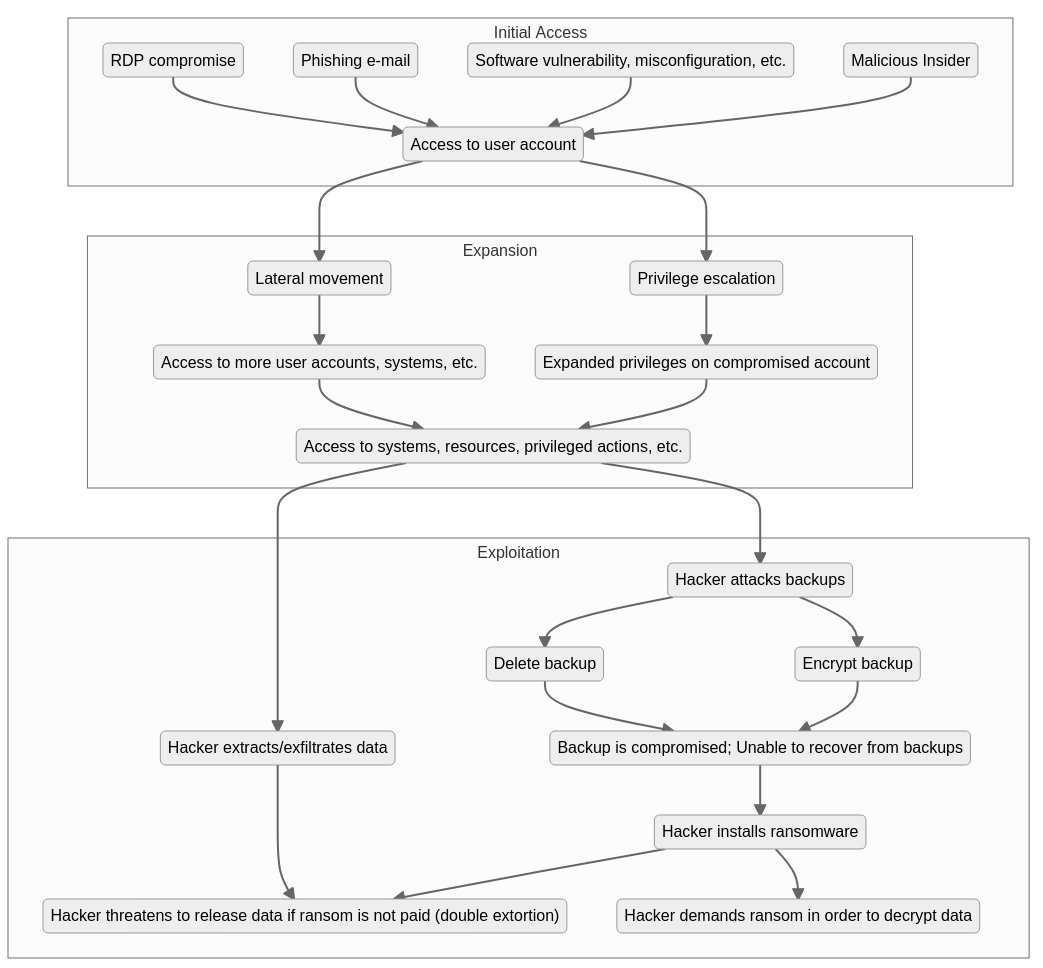
\includegraphics[width=.9\linewidth]{figures/attack_anatomy.png}
    \caption{Illustration of the anatomy of a cyber attack}
    \label{fig:attack_anatomy}
\end{figure}

\subsection{Attacks against backups}
%[TODO] var her 19.mai

Since \gls{backup}s are an essential part of being able to recover from a ransomware attack,
hackers will often try to destroy their victim's backups before encrypting files. Backups are explored in detail in section \ref{Backup}
In this section, we will outline a few possible attack vectors 
against the backups themselves that could try to make them useless.

The simplest way of destroying backups is to simply delete them.
By deleting an organization's backup, hackers can deny recovery, 
which can increase the chance that the organization pays the ransom.

A potential method of corrupting an organization's backups could be to slowly encrypt
the data that is being backed up.
Over time, the backups would be overwritten with invalid data,
making them useless by the time the ransomware is deployed.

A hacker could potentially exfiltrate data from backups.
By encrypting data before backing it up, this risk can be mitigated.
If a hacker exfiltrates encrypted data,
they will not be able to read it without having access to the encryption key used.
    
\section{Backup} \label{Backup}
Faced with ransomware attacks and malicious actors that target the data of organisations, securing that data is essential. It is a fact of living in a digital, interconnected world that malicious actors will attempt to target any data that is available. Face with that risk keeping backups is an important security control.

According to Sjaak Laan, "Managing security is all about managing risks" \cite{laan_it_2017}. Faced with any type of risk, senior management has the option between risk acceptance, avoidance, transfer, and mitigation. While having no data stored digitally, or completely disconnecting all systems from the outside world would be considered avoidance, and some sort of insurance would be considered risk transfer (although almost half of victim organisations that has cyber insurance only got a portion of the losses covered \cite{noauthor_new_nodate}.) An effective backup solution would be an effective risk mitigation technique. 

Laan defines a backup as copies of data, used to restore data to a previous state in case of data loss, data corruption, or a disaster recovery situation. Laan argues that a backup older than a few weeks is of little use, as old, outdated data is probably not very useful for a company in an emergency. The archiving of older data for compliance should be done separately from backups (but should be backed up also) \cite{laan_it_2017}.

Recovery is the process of restoring files from a backup, and is an essential part of any plan to mitigate data loss risk. A backup without a good plan for recovery loses a lot of its use. Recovery should also include procedures for spinning up new VMs as in case of a ransomware attack it would be fair to assume the network to be infected.

In his book "Infrastructure as Code," Kief Morris \cite{morris_infrastructure_2020} argues that in the cloud age organisations should plan for disaster recovery continuously, for example by using the same tools to recover from a disastrous event as an organisation uses to provision and change infrastructure. Recovering from complete disaster should according to him be as easy as anything else. Restoring from a backup in the cloud, and accessing the necessary data on fresh, secure VMs is principal in cloud infrastructure design.

\subsection{Types of backup} \label{Backup Strategies}
There are a few main types of backups that are commonly used.
These are \emph{full}, \emph{differential} and \emph{incremental} backups.
A brief description of each type of backup follows below.

\subsubsection{Full backup}

One of the most straightforward types of backup.
In a full backup, all the data is backed up at once.
Depending on the amount of data, this can take a long time,
and may require a lot of storage.
Recovering from a full backup is usually very simple.
All one needs to do is load the disk containing the backup,
and start the recovery process.

Full backups only require one backup medium 
(unless the amount of data is very large, in which case it needs to be distributed).

\subsubsection{Differential backup}

Differential backups are built upon an existing full backup.
They work by only backing up the changes made since the last full backup, 
instead of backing up all the data.
Since the amount of data changed is generally much lower than the total amount of data,
this is usually faster than doing a full backup every time.

Differential backups require at least two disks, one for the full backup and one for the changes.
Recovery can be done by loading the full backup first, and then the changes.
Recovery from a differential backup is generally slower than from a full backup, but faster than from an incremental backup.

\subsubsection{Incremental backup}

Incremental backups are similar to differential backups,
in that only changes since the last full backup are backed up.
However, unlike differential backups, where all changes since the last full backup are stored,
incremental backups store only changes since the previous \emph{backup activity} (full or incremental).

Recovery from incremental backups consist of first loading the full backup,
then all the incremental backups in order.
This can be a time consuming and complicated process, 
especially if done using physical drives.
Some cloud platforms automate this process,
making it both fast and easy.

\subsection{Database backup}

There are several ways to back up databases.
Many databases support a way to to generate a series of SQL statements that recreate the database.
This is called a \emph{database dump}.
To recover from a dump, the SQL statements are simply run by the database engine.
% This type of backup essentially only stores the data in the database.

Another way to back up a database is to make a backup of the entire virtual machine the database is running on.
This consumes more storage than a dump, but can potentially be faster to recover from,
since software and configuration files are backed up alongside the data.

%-------

\section{The Azure cloud platform}

Microsoft Azure is one of the largest cloud platforms on the market \cite{richter_amazon_2022}.
The platform provides a number of services to organisations that wish to move to the cloud.

% Azure provides a number of relevant security features for creating a secure and effective backup solution. Access to backup data can be protected by role based access control, and multi user authorization, and is only available through Recovery Services vault and Backup vault. 



\subsection{Azure Backup} \label{AZBackup}
Azure Backup is the go-to backup service in Azure. It aims to "provide simple, secure, and cost-effective solutions" for backing up, and recovering data from the Microsoft Azure cloud \cite{v-amallick_what_nodate}.
The service supports a number of services and storage solutions, and the list appears to be expanding.
One month into this project for example, it was announced that Azure Backup now supports the managed Azure Database for PostgreSQL-service that is in the scope of our project, with the release of Azure PostgreSQL backup with long-term retention in February 2022 \cite{noauthor_generally_nodate}. 

Azure Backup offers a number of benefits, according to the Azure documentation \cite{v-amallick_what_nodate}.
The data stored in Azure backup is not directly available to the attacker \cite{terrylanfear_azure_nodate}. 
Protecting backup vaults with Role Based Access Controls (RBAC) is also an important part of protecting the data from ransomware \cite{v-amallick_faq_nodate}. 
RBAC will be discussed in more detail shortly, in section \ref{theory:RBAC}.
%Azure Monitor provides provides ways to monitor actions relating to backups.

Azure Backup has support for backing up a number of different resources. There is support for backing up files, folders, and system state of on-premise systems by using Microsoft Azure Recovery Services (MARS) agent \cite{v-amallick_manage_nodate}.

Backup items are stored in vaults, either a Recovery Services vault, or a Backup vault. Vaults are online storage entities in Azure. According to Microsoft they are designed to make it easier to manage the backed up data. Vaults offer monitoring of the backup data, and configuration of things such as redundancy. Each vault holds data, "such as backup copies, recovery points, and backup policies." \cite{v-amallick_architecture_nodate}

\subsubsection{Recovery Services Vault} \label{theory:rsv}
A Recovery Services vault (RSV) is a type of management entity for backups in Azure.
It is a newer version of Backup vaults with a number of additional features. 
Since its release in 2016, it has been supported with security features like soft delete, Cross Region Restore, and Multi-user authorization \cite{v-amallick_overview_nodate-1}. 
The Multi-user authorization and soft delete features are discussed in sections \ref{MUAtheory} and \ref{Soft Delete} respectively.

Vaults also support a variety of data redundancy tiers (\ref{theory:redundancy-tiers}),
which provide different ways to replicate data across data centers.

The services supported by Recovery Services vaults, according to Microsoft \cite{v-amallick_overview_nodate-1}, are:
\begin{itemize}
    \item Azure Virtual machines
    \item SQL in Azure VMs
    \item Azure Files (Azure Storage)
    \item SAP HANA databases in Azure VMs
    \item Azure Backup server
    \item Azure Backup Agent
    \item DPM
\end{itemize} 

Backup items are held locally, in a storage account, for a while before being transferred to the vault.
Transferring items to a vault can take several hours, but it happens automatically. 
\subsubsection{Backup Vault}
Backup vaults are the older version of recovery services vaults, and therefore offer less functionality.
There is no support for soft delete, Multi-user authorization, or other newer security features.
In 2017 Microsoft announced in a blog post that they would support "seamless upgrade of classic Backup or Site Recovery vaults to ARM based Recovery Services vaults. " \cite{somendra_upgrade_2017}

Backup vaults are still supported in Azure backup to this day,
but its primary use is to be "a storage entity in Azure that houses backup data for certain newer workloads that Azure Backup supports" \cite{noauthor_overview_nodate}.
This includes Azure Database for PostgreSQL servers, and other newer workloads:

\begin{itemize}
    \item Azure Database for PostgreSQL servers
    \item Azure Blobs (Azure Storage)
    \item Azure Disks
    \item Kubernetes Service (Preview)
    \item AVS Virtual machines (preview)
\end{itemize}

\subsubsection{Azure snapshots}
% Building blocks for azure backup

A snapshot typically refers to a read-only point-in-time copy of something,
for example a virtual machine or a hard drive.
Unlike file based backups which store only data files,
snapshots store additional state. %like what

Azure snapshots are read-only copies of a managed virtual hard disk (VHD). % double check managed
These snapshots can be used for backup and recovery purposes.
The snapshots can then be recovered to a new VHD.
If the snapshotted disk was an operating system disk,
it's possible to create a new VM directly from the snapshot.

Azure provides two types of snapshots, full and incremental.
These are essentially implementations of full and incremental backups (see \ref{Backup Strategies}).
A full snapshot makes a copy of the entire disk, 
while an incremental snapshot only makes a copy of the changes since the last snapshot.
Traditionally, incremental snapshots provide faster backup speeds, 
at the cost of a slower and more complex recovery process.
This is not the case with Azure's snapshots.
According to Microsoft blog, 
recovery is almost as fast from incremental snapshots as with full snapshots,
and recovery time is constant no matter how many snapshots are used
\cite{noauthor_incremental_nodate}.
Incremental snapshots in Azure can be deleted without invalidating newer snapshots.

\subsubsection{Azure data redundancy tiers} \label{theory:redundancy-tiers}

Azure provides several tiers of redundancy for data stored in certain Azure services.
These tiers provide different ways of replicating data,
the goal being to prevent data loss in case an incident occurs.
The tiers are described below in order of increasing price \cite{tamram_data_nodate}.

Locally redundant storage (LRS) stores 3 copies of the data, in the same data center.
Zone-redundant storage (ZRS) stores 3 copies of the data, in different data centers in the same region (one copy per data center).
Geo-redundant storage (GRS) replicates LRS from the primary region to a different secondary region ($2 \times 3$ copies).
Geo-zone-redundant storage (GZRS) combines ZRS and LRS. Data in the primary region is stored in ZRS, while data in the secondary region is stored in LRS.

\subsection{Role based access control (RBAC)} \label{theory:RBAC}
In Azure, access to resources is only granted when an identity can be authenticated, 
and it has been assigned the correct permissions. Identites are essentially what seperates different users and resources from each other. Each user has a different identity that is used in RBAC to grant them the access they need. 
According to Modi, in \textit{Azure for Architects}, this is known as authorization, or more commonly as Role-Based Access Control, or RBAC \cite{modi_azure_2019}.
"RBAC in Azure refers to the assigning of permissions to identities within a scope. 
The scope could be a subscription, a resource group, or individual resources."

RBAC helps control which users have access to which resources,
with as much granularity as is needed to segregate permissions within an organisation as well as a single team.
In general it is considered best-practice to only provide the least level of access necessary to perform a task.
Modi argues that separating access between team-members helps ensure both security,
as well as keeping team-members feeling responsible for their jobs as they may be the 
only ones with a necessary level of access to perform some tasks. 
 
RBAC has been an important concept of security administrations since its formalization in 1992, by by David Ferraiolo and Rick Kuhn.
It is the predominant model of advanced access control according to NIST.
One of the advantages of RBAC is that security is managed at a level to closely corresponds to an organization's structure.
Many important security features,
such as multi-user authentication, and the zero-trust model builds upon RBAC.
% , and RBAC is in that way essential for this project.

\subsection{Multi-User Authorization (MUA)} \label{MUAtheory}

While RBAC is useful for administrating access to Azure resources,
it may become useless if an attacker is able to perform a \gls{privilege escalation} attack.
Destructive actions will still trigger alerts for system administrators,
but by the time these are initiated, it may be too late.

Multi-user authorization is a relatively new security feature in Azure which can mitigate this risk.
MUA allows the use of a Resource Guard to protect Recovery Services Vaults in Azure (\ref{theory:rsv}).
This Resource Guard is owned by a different user (the security administrator) in Azure.
The owner of the resource needs to request permission from the security administrator,
in order to to perform destructive actions on the resource \cite{noauthor_protect_2021}.
As a result, no person is solely in control of any task that may be destructive to the backup data.
This can greatly reduce the risk of data loss in case one of the administrator accounts is compromised.

The actions supported by MUA as of this report is:
\begin{itemize}
    \item Disable soft delete
    \item Disable MUA protection	
    \item Modify backup policy	
    \item Modify protection	
    \item Stop protection	
    \item Change MARS security PIN	
\end{itemize}

\subsection{Soft delete} \label{Soft Delete}

Soft delete is a security feature for Azure Backup or Azure Storage Blobs.
When soft delete is enabled, data that is deleted is not removed immediately. 
Instead it is retained for 14 days before being permanently deleted. 
During this time, it is possible to "undelete" the data.
Soft delete is enabled for Recovery Services Vaults by default.

\subsection{Azure Monitor}

Azure Monitor is a service that monitors resources and services in Azure.
If certain actions or events are detected, Azure Monitor can issue alerts to the relevant administrators.
An example is the \textit{Delete Backup Data} alert, which is sent out if any backup data is deleted.
Alerts are either sent to the Azure Monitor view or via email, if it is serious enough.
According to the documentation, certain alerts relating to Azure Backup are sent via email automatically
\cite{v-amallick_monitoring_nodate}.
Custom alert rules can also be configured.


\subsection{Interacting with Azure} 

Azure provides three main methods of interaction:
\begin{itemize}
    \item Azure Portal\\
    The Azure Portal is a graphical interface for managing an Azure environment.
    The Portal is generally quite user friendly.
    \item Azure CLI\\
    The Azure CLI is a set of commands which can be used to manage an Azure Environment.
    The CLI can be accessed through the Azure Cloud Shell, which is a type of console in the Azure Portal.
    The CLI makes it possible to make scripts to automate processes.
    \item Infrastructure as Code (IaC)\\
    Infrastructure as Code is an approach to infrastructure management where resources are
    declared and configured programmatically.
    This can improve stability and reduce maintenance.
    IaC can be implemented using Azure Resource Manager templates,
    or by using third-party tools like Terraform \cite{nishanil_infrastructure_nodate}. 
\end{itemize}

\subsection{Azure Blob Storage} \label{theory:blobs}

Azure Blob Storage is a storage solution in Azure which is optimized for large amounts of data \cite{tamram_introduction_nodate}. 


\section{ClickHouse} \label{Clickhouse}

\subsection{Introduction to ClickHouse}
% [TODO] Fylle ut

ClickHouse is a database used for Online Analytical Processing (OLAP).
It is highly optimized for certain types of workloads,
and is able to process large amounts of data in an efficient manner \cite{noauthor_what_nodate-2}.

ClickHouse runs as a server on a virtual machine,
which can be accessed using the program \texttt{clickhouse-client}.
ClickHouse uses SQL as its query language.

\subsection{Backup solutions for ClickHouse} \label{theory:ch-solutions}

According to the ClickHouse Documentation, there is no universal backup solution for ClickHouse,
but the documentation contains a few different suggested solutions \cite{noauthor_data_nodate}.
In this section, we will provide a short summary of the solutions listed in the documentation.

\begin{itemize}
    \item Duplicating Source Data Somewhere Else \\
    A program such as Apache Kafka can be used to serve a stream of data as input to ClickHouse.
    This stream can be forked and diverted to send data to backup storage at the same time as it is sent to ClickHouse.
    \item Filesystem Snapshots \\
    Some filesystems like ZFS support making \emph{snapshots} of the filesystem's state.
    These snapshots can then be sent to an external storage solution.
    \item clickhouse-copier \\
    clickhouse-copier is a tool that can be used to copy data between ClickHouse clusters.
    Originally intended for petabyte-sized databases.
    \item Manipulations with Parts \\
    A local copy of a table can be made with ClickHouse's built-in \texttt{ALTER TABLE FREEZE} query.
    The copy can be exported with a program like \texttt{rsync}.
    \item clickhouse-backup  \label{theory:chbk} \\
    clickhouse-backup is a tool that automates the \emph{manipulations with parts} approach.
    The tool is installed on the same server as ClickHouse.
    It can store backups locally or on a remote server, using various storage methods,
    like Azure Blob Storage or AWS S3 object storage.
\end{itemize}

\subsection{Backup solutions for ClickHouse in Azure}

Azure provides tools for backing up data.
These are not mentioned in the ClickHouse documentation,
since they are not specific to ClickHouse.
Azure Backup supports backing up individual virtual machines as described in \ref{AZBackup}.
This feature can be used to back up the VM running ClickHouse.

%-----------

\section{PostgreSQL} \label{Postgres}

\subsection{Introduction to PostgreSQL}
PostgreSQL is an open-source relational database management system (RDBMS). It is suited for operations requiring complex SQL queries, and provides functionality enabling data analysis. Azure has its own hosted solution called Azure Database for PostgreSQL, which automates maintenance, patching, and updates \cite{noauthor_azure_nodate}. It also allows effortlessly scaling the database size and computing.

 There are only a few backup options that are relevant to look into when working with a managed PostgreSQL instance hosted in Azure. This short introduction will also include frequently seen practices for unmanaged instances of PostgreSQL before narrowing the focus into managed ones hosted on Azure.

% TODO: Say something about the managed Postgres service in Azure

\subsection{Backup solutions for PostgreSQL}

One recovery option for protecting backup could be removable storage.
This will however not be the focus when exploring options for a ransomware-resistant backup architecture.
 
Some options for backing up a PostgreSQL database include extraction of data using the pg{\_}dump command. This way one could back up data off-site for increased security by air-gapping, although setting this up in such a way that RTO and RPO are met can prove challenging. Moreover, a backup restore from a remote server takes longer time than a local copy. 

\subsection{Backup solutions for PostgreSQL in Azure}

%-----------
\subsubsection{Azure Backup} \label{theory:PITR}
Azure Database for PostgreSQL backup has long-term retention in Backup Vaults. A backup vault is a storage entity housing backup data in Azure \cite{v-amallick_overview_nodate}. It requires connecting to a Key Vault to integrate with the database instance that will be backed up. Azure Key Vault stores and allows accessing secrets \cite{noauthor_key_nodate}. Examples of secrets could be API keys, passwords, certificates, or cryptographic keys. In this case, it is the database connection string.

The Backup Vault has long-term retention of up to 10 years. It also allows configuration and granular control allowing for a backup policy that complies with the organisations needs.

%A distinction here has to be made between Azure Database for PostgreSQL backup and the native backup solution offered by Azure PostgreSQL. The main difference between the two is the period of time that data is retained and the customization options. Azure Database for PostgreSQL backup has long-term retention of up to 10 years. It also allows configuration and granular control allowing for a backup policy that complies with the organisations needs.
%En del av dette under må omskrives med egne ord, noe er tatt ordrett fra dokumentasjonen.
%In addition to this there are multiple features such as scheduled and on-demand backups at database level. It is also possible to create a backup of the PostgreSQL server database to another server or to Azure blob storage. 
%Compartmentalisation and isolation to a certain extent also follow with Azure Database for PostgreSQL where backups are stored in separate security and fault domains. 
% Explain security and fault domains here.
%Lastly, use of pg\_dump can allows for restoration across database versions.

\subsubsection{Point-in-time-Restore} \label{theory:PITR}
In contrast, the built-in Point-in-time-Restore (PITR) solution has a default retention of only 7 days, which can be set to a maximum of 35 days. If the server size is up to 4TB the native solution operates on two differential backups a day and a full backup once a week. If larger than 4TB and up to 16TB, the solution operates on snapshot based differential backup, with three snapshots performed in a day.
% Her må det omskrives litt der det ligner for mye på docs fra lenken under.
% https://docs.microsoft.com/en-us/azure/backup/backup-azure-database-postgresql-overview

The built-in backup solution and the Azure Database for PostgreSQL backup can operate simultaneously. 

\section{Security Best Practices} \label{BestStrat}

\subsection{Principle of least privilege}
When assigning permissions to users and processes to access resources in an organisation, it is considered best practice according to the principle of least privilege to only give the minimum level of access needed at any given time. For example doing menial tasks like checking emails and browsing the internet should not be done while accessing a system as administrator. In modern systems architecture the role of system administrator should not be used instead, access should be provided only to the resources a user needs at at given time \cite{ramel_anatomy_nodate}.
In Azure, this is implemented with RBAC (\ref{theory:RBAC}).

\subsection{Zero trust}
One of the modern mainstays of cybersecurity and infrastructure security is the Zero Trust model.
The National institute of standards (NIST) special publication 800-207 provides the following definition: 
"Zero trust provides a collection of concepts and ideas designed to minimize uncertainty in enforcing accurate,
least privilege per-request access decisions in information systems and services in the face of a network viewed as compromised." 
\cite{cybersecurity_and_infrastructure_security_agency_cisa_2021} 

This definition says that one should view the network as compromised,
and as such bear that in mind for every decision made when designing the network.
The alternative, assuming a network or system is not compromised,
has disastrous consequences if this assumption is incorrect.
This can be exemplified by Ramel's retelling of a ransomware attack where the cause of the breach was an administrator logging in to a compromised system to perform mundane tasks with admin privileges \cite{ramel_anatomy_nodate}. The attacker would not have been able to gain admin rights if it hadn't been for the unnecessary use of the administrator account. \label{ZeroTrust}

Zero Trust architecture is described by CISA as fundamentally different from prior models,
and one that will require a holistic change in the way an organisation thinks about its cybersecurity controls,
but also its philosophy and culture around cybersecurity. 

The core concept of a Zero Trust architecture is that security is no longer perimeter-based,
and that there is an implicit assumed threat in any network.
Therefore the security model focuses on data and service protection,
and only providing the minimal level of access to resources and data when, and only when, that access is needed.
Trust and access must always be continually evaluated,
and an attacker won't have free reign of all resources once inside a network.
The model aims to hinder the unauthorized lateral movement of attackers inside networks once the perimeter is breached 
\cite{rose_zero_2020}. 

The same source describes a number of factors that may enable a system to grant or deny access to a resource. A trust algorithm uses these factors to make a decision on whether or not it is likely that the request is legitimate, and denies it if it is not likely. The trust algorithm can be run multiple times during a session to continually confirm the legitimacy of the access given to a subject. 
 
% \subsection{Automation solutions} \label{IaC}
% Infrastructure as Code is a broad subject, and far beyond the general scope of this project, however some key aspects should be mentioned. Morris' book on the subject is already mentioned in this report, and it supports the claims in this subsection. 
% 
% Whilst designing infrastructure solutions in the cloud system architects should attempt to leverage any and all benefits of a cloud environment if they can. One of these benefits that Morris mentions early and often is to assume systems are unreliable. In essence, an organisation can't expect a VM to remain stable and running into eternity. This, he argues, means that systems should never be modified after creation. 
% 
% It ties into another key principle of his, which is to make everything reproducible. That means that any infrastructure in a system should be able to be rebuilt completely and still function as intended and according to the needs of the organisation. 
% 
% The argument for automation is supported by security architect in CheckPoint, Pål Aaserudseter, who says in an interview with digi.no that by 2025, 99\% of security incidents will be caused by human error. \cite{samsonsen_sikkerhetsarkitekt_2022} Norkarts data leak that was reported on the 10th of may 2022, is an example of this, as the cause of the breach was a misconfigured firewall. \cite{samsonsen_persondata_2022} 

%-----------
